\chapter*{Rilevamento della frequenza fondamentale}\label{cap:rilevamento_frequenza}

L'algoritmo utilizzato per rilevare la frequenza fondamentale è l'algoritmo \emph{Harmonic Product Spectrum}, abbreviato dall'acronimo \emph{HPS}.
Tale metodo sfrutta il fatto che quando viene suonata una nota con uno strumento musicale, l'energia del suono si concentra principalmente nella frequenza fondamentale e nelle sue armoniche, cioè i suoi multipli interi.

L'algoritmo HPS moltiplica lo spettro del segnale con un numero \emph{K-1} di versioni differenti dello spettro.
Le diverse versioni sono ottenute sotto-campionando lo spettro originale con i diversi fattori compresi tra 2 e K.
La formula \ref{formula:hps_prod} descrive la prima parte di questo algoritmo per un generico spettro X($\omega$) e un generico valore \emph{K}.

	\begin{equation}\label{formula:hps_prod}
		Y(\omega) = \prod_{i=1}^K \left | X(\omega i) \right |
	\end{equation}

Una volta ottenuto il prodotto, la frequenza fondamentale viene calcolata come ascissa del massimo della funzione risultante. 
La formula \ref{formula:hps_max} descrive questo secondo passaggio.

	\begin{equation}\label{formula:hps_max}
		Y_{f0} = \max_{\omega_i} Y \left(\omega_i \right )
	\end{equation}

La figura \ref{fig:HPS} chiarifica l'effetto dell'algoritmo. 
Dal momento che l'energia è concentrata nelle armoniche, le versioni scalate dei segnali avranno comunque un picco nella frequenza fondamentale. 
Ciò non si verifica con le altre armoniche, che in alcune versioni del segnale verranno moltiplicate per valori piuttosto bassi. 
Questo fatto comporta una riduzione del picco attorno a quelle frequenze. 
Il risultato del prodotto tra le diverse versioni scalate dei segnali si può vedere nella parte destra della figura. 
Il segnale risultante avrà un unico picco nella frequenza fondamentale.

	\begin{figure}[h]
	  \begin{center} 
	    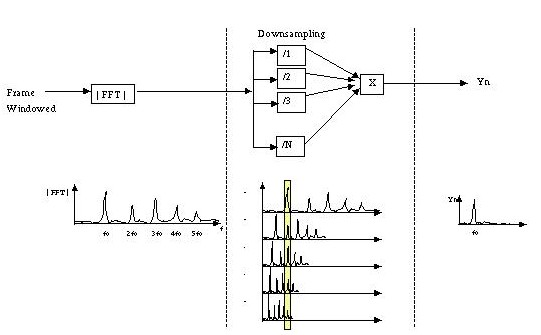
\includegraphics[width=\textwidth*\real{0.9}]{images/ch_04/processo.jpg}
	  \end{center} 
	  \caption{\textit{Metodo HPS}}  
	  \label{fig:HPS}
	\end{figure}

Nel contesto dell'accordatore, il metodo è stato applicato moltiplicando il segnale originale con le prime versioni scalate del segnale.
L'algoritmo, inoltre, prevede di usare la tecnica di zero-padding sui segnali scalati in modo che essi vengano adattati alla lunghezza del vettore originale. 
Questa operazione è stata evitata troncando tutte le versioni dei vettori da scalare al numero di elementi del vettore più corto.
Ciò è stato possibile dal momento che la frequenza fondamentale più alta della chitarra è di 329.63 hz, corrispondente al \mbox{mi} alto.
Il segnale più corto tra quelli da moltiplicare è quello scalato con il fattore maggiore, cioè 5.
La frequenza massima del segnale scalato si ottiene dividendo la frequenza massima del segnale, cioè 4 kHz per il fattore di compressione, 5. 
Il risultato, 800 hz, è ben oltre il doppio dell'ottava della nota più acuta suonata dalla chitarra, quindi questa operazione è realizzata senza nessun rischio per l'individuazione della frequenza fondamentale.

L'operazione di ricerca del massimo è calcolata su una versione ulteriormente finestrata della funzione prodotto. 
In particolare, vengono escluse le frequenze inferiori ai 40 hz in quanto il rumore in questo range è molto intenso, come discusso nel capitolo \ref{cap:rumore}.
La generalità dell'algoritmo di ricerca della frequenza non viene penalizzata, in quanto il minore delle frequenze fondamentali delle note della chitarra è di 82.41 hz, corrispondente alla sesta corda, cioè al \mbox{mi} grave.

Il risultato del doppio finestramento può essere paragonato all'applicazione di un filtro passa-banda ideale sul segnale prodotto, con intervallo di frequenze pari a [40,800] hz.
Si è potuto utilizzare un filtro ideale in quanto tutte le operazioni effettuate riguardano il dominio delle frequenze.
Il segnale nel dominio del tempo, quindi, non deve essere ricostruito.




